%!TEX root = ../thesis.tex
%*******************************************************************************
%*********************************** First Chapter *****************************
%*******************************************************************************

\chapter{Introduction}  %Title of the First Chapter

\ifpdf
\graphicspath{{Chapter1/Figs/Raster/}{Chapter1/Figs/PDF/}{Chapter1/Figs/}}
\else
\graphicspath{{Chapter1/Figs/Vector/}{Chapter1/Figs/}}
\fi

%********************************** %First Section  **************************************
%\section{The Shoot Apical Meristem of \textit{Arabidopsis thaliana}} %Section - 1.1 

% first letter Z is for Acronyms 
% first letter A is for Roman symbols
% first letter G is for Greek Symbols
% first letter G is for Greek Symbols
% first letter G is for Greek Symbols
% first letter X is for Other Symbols
% first letter R is for superscripts
% first letter S is for subscripts
\nomenclature[z-AT]{AT}{\textit{Arabidopsis thaliana}}
\nomenclature[z-SAM]{SAM}{Shoot apical meristem}                               
\nomenclature[z-RAM]{RAM}{Root apical meristem}                               
\nomenclature[z-CZ]{CZ}{Central zone. The region harboring stem cells in the SAM.}                                                                        
\nomenclature[z-PZ]{PZ}{Peripheral zone}                                          
\nomenclature[z-OC]{OC}{Organising center}                        
\nomenclature[z-RM]{RM}{Rib meristem}                                          
\nomenclature[z-L1]{L1}{Layer-1. The outermost cell layer of the SAM.}
\nomenclature[z-L2]{L2}{Layer-2. See L1.}
\nomenclature[z-L3]{L3+}{Layer-3 and other deep-tissue cells. See L1.}

\nomenclature[z-GRN]{GRN}{Gene regulatory network}
\nomenclature[z-ODE]{ODE}{Ordinary differential equation}
\nomenclature[z-SDE]{SDE}{Stochastic differential equation}

\nomenclature[z-CLV3]{CLV3}{CLAVATA-3}                                         
\nomenclature[z-WUS]{WUS}{WUSCHEL}                                             
\nomenclature[z-KAN]{KAN1}{KANADI-1}                                           
\nomenclature[z-STM]{STM}{Shoot meristemless}

\nomenclature[z-dsRED]{dsRED}{Red fluorescent protein. Used for nuclear CLV3
  staining.}
\nomenclature[z-YFP]{YFP}{Yellow fluorescent protein. Used for membrane
  staining.}
\nomenclature[z-SLCU]{SLCU}{Sainsbury Laboratory at the University of Cambridge}

%********************************** %Second Section  *************************************
\section{The shoot apical meristem of \textit{Arabidopsis thaliana}} %Section - 1.2
\label{sec:arabidopsis}
% The Shoot and the Root
Plant stem cells are organised by two developing centra -- the Shoot Apical
Meristem (SAM) and the Root Apical Meristem (RAM). The SAM is the region
responsible for development of all aerial organs in the plant, and relies on a
tighly orchestrated regulatory system in order to ensure a stable and functional
developmental process. This includes
aspects of cell proliferation and specification, as well as an ability of the plant to
maintain and regulate the stem cell identity of the cells at the very apex of
the shoot~\cite{clark2001cell}. As opposed to the RAM, which has two stem cell pools in the
inside of the root, the SAM maintains a single stem cell pool centered at the
apex. It also lacks the root's cap, which protects the stem cells on the inside
of the root, whereas these in the shoot are directly exposed to the plant's
surroundings. Because of its highly exposed stem cell niche, the plant's
regulatory system must therefore be organised in such a way that it can withstand  
significant perturbations, both due to molecular noise and changes in environmental
conditions~\cite{heidstra2014plant}.

% What stem cells do
The stem cells at the SAM contribute to the development of new organs and
tissue by dividing frequently at the top and from there 
mechanically being pushed out of the apex in order to differentiate, as
illustrated in \cref{fig:structure}. The steady
maintenance of the stem cell niche allows for a constant production and supply
of cells that the plant utilises during both growth and repair of damaged
tissue, and is therefore completely essential for the plants
survival~\cite{heidstra2014plant}.

\begin{figure}[H]
  \centering
  \begin{minipage}{0.25\textwidth}
    \centering
    
\includegraphics[width=.95\textwidth]{arabidopsis.pdf}
  \end{minipage}\hfill
  \begin{minipage}{.75\textwidth}
    \centering
    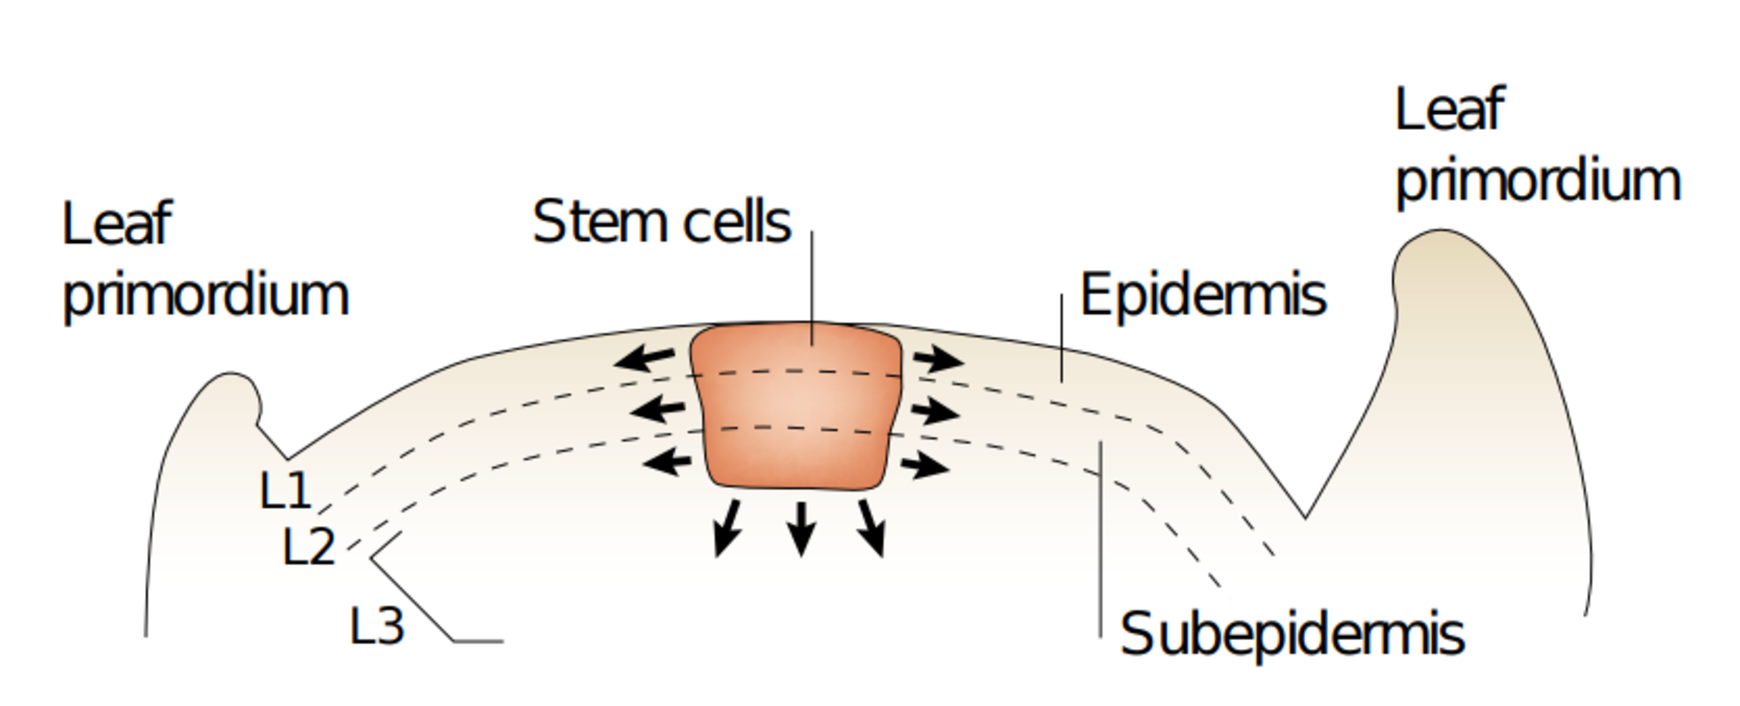
\includegraphics[width=.95\textwidth]{structure.pdf} % second figure itself
  \end{minipage}
  \caption[Graphical illustration of \textit{Arabidopsis thaliana} and the
  \textit{Shoot Apical Meristem}]{Graphical illustration of model plant \textit{Arabidopsis
      thaliana} and the shoot stem cell niche. The SAM consists of a
    dome-like domain where a small pool of stem cells are maintained
    throughout the life-span of the plant. Over the course of development,
    the cells are continously pushed out of the stem cell niche out into the
    stem or periphery, where they differentiate. Structurally, the shoot is
    separated into three distinct layers that are of functional
    importance, here denoted L1, L2 and L3. Figure adapted from
    Clark~\cite{clark2001cell}.}
  \label{fig:structure}
\end{figure}

% Structure composition of the plant
In a simple outline of the SAM, its structure can be said to consist of four core regions:
1) The \textit{central zone} (CZ), which harbors the aerial \textit{stem cell niche} 
of the plant; 2) The \textit{organising center} (OC), which is located beneath
the CZ and acts as a signalling hub for many of the genes driving development in
ot he SAM; 3) The
\textit{peripheral zone} (PZ), where cells form organs and new tissue through
differentiation; and 4) the \textit{rib meristem}, which make up the bulk of the
SAM, and consist of the cells making up the stem. In addition to these regions,
the SAM is also often separated 
into the different layers of the dermis, denoted L1 for the epidermal
layer, L2 for the sub-epidermal layer, and L3 for the inner ground
and vascular tissues. For cells in both L1 and L2, proliferation happens
orthogonally to the shoot surface, i.e.\ so that cell lineages are preserved
within the L1 or L2 correspondingly, with few exceptions. In contrast,
this is not the case for the L3, where 
cells more freely can divide in all directions~\cite{scheres2007stem}. In
addition, it has been suggested
that the epidermis is involved in both promoting and restricting shoot
development~\cite{gruel2016epidermis}, adding to the
notion of coordination and regulation between the different cell layers in order
to accurately direct plant growth. 
% Rewrite last sentence?

\section{Modelling biological systems} %Section - 1.2
\label{sec:modelling}
% Systems biology
From a theoretical point of view, organismal development can be
considered in the framework of being a \textit{complex system}. This is
particularly useful in understanding the molecular pathways that ultimately end
up determining cellular functonality and the general development of organisms.
In a \textit{systems biology} setting, molecular and mechanical interactions are
treated as abstract entities, each representing some fundamental part of the
whole system in question, much like how machinery can be explained by its
separate cogs and gears working together. Specifically in a molecular setting,
the descriptive approach is commonly through \textit{Gene Regulatory Networks}
(GRNs), wherein each component represents some molecular aspect of the system
that is involved in producing expression levels of mRNA, proteins and
hormones~\cite{kitano2002systems}.

% Gene regulatory networks and mathematical modelling
Dynamics of GRNs are commonly understood both through analytical and computational means,
where in the latter computer-generated models provide as a modern tool for
better understanding the complex nature of many biological systems. Typically,
reaction kinetics are modelled using various types of \textit{Ordinary
  Differential Equations} (ODEs), although due to the vast amount of processing
power available in the modern day, many recent studies also utilise
traditionally more demanding resources such as \textit{Stochastic Differential
  Equations} (SDEs). These also take into account the inherently random nature of molecular
motions, interactions, and processes in order to capture dynamical features that
deterministic versions cannot. For example, the ability of a cell to
probabilistically change state depending on its environement, e.g.
when commiting to producing a certain protein or deciding to undergo apoptosis,
can be the difference between life and death for the organism. Utilising the
inherent noise of microscopic 
systems, cells have indeed been repeatedly shown to probabilistically tune their
responses~\cite{locke2011stochastic,losick2008stochasticity,mennstochastic}, showcasing the need of stochastic modelling for such types of
phenomena.

In addition to stochasticity, the increase in computability has also allowed for
the feasibility of spatiotemporal modelling, where systems are evaluated not only
in a static context, but also in changing settings. This has allowed insights
into how the distribution of gene expression varies over time, and how organisms
orchestrate their developmental machinery such that organs and other types of
tissue are developed at the right time~\cite{ietswaart2015spatiotemporal}. 

% Model prediction and verification 
Computer models in general have two separate aims: exploration and validation.
In the former case, computer simulations can be the core for designing
experiments, where hypotheses from observed theoretical phenomena
can be experimentally tested. In the latter, models are established in order to
support hypotheses surrounding experimental findings, and can directly guide
experiments through the identification possible mechanism behind an observed
behaviour. The interplay between models and experiments, exploration and
validation, causes the iterative process displayed in~\cref{fig:expl_val},
through which computational models and direct experiments work in conjunction to further
common knowledge.
\begin{figure}[H]
  \centering
  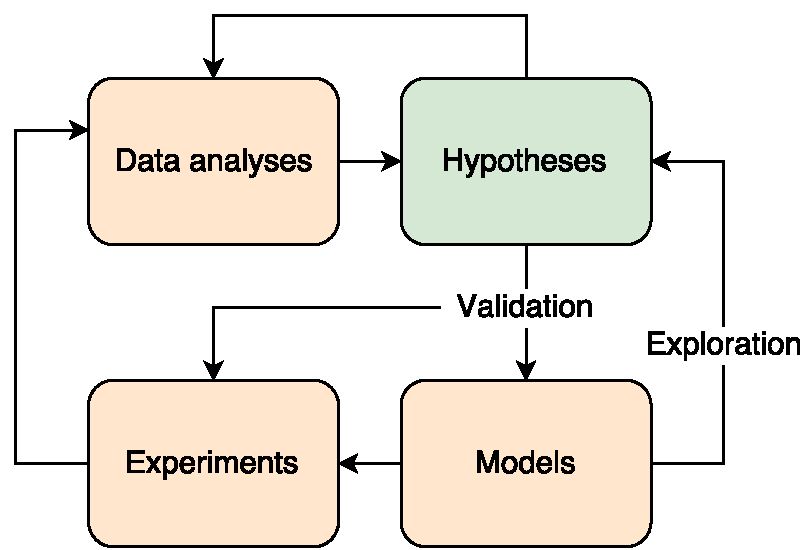
\includegraphics[width=.5\textwidth]{exploration_validation.pdf}
  \caption[Modelling biological systems: an illustration]{Flowchart describing
    the work process in biological modelling. Investigations are driven by
    hypotheses, typically based on various types of data, or by the outcome of
    model simulations. Exploration or verification of these through either
    models or experiments in turn foster new hypotheses, creating an iterative
    process of continued research.}  
  \label{fig:expl_val}
\end{figure}

\section{Regulatory Mechanics of Plant Stem Cells} %Section - 1.2
\subsection{Molecular tuning determines cell phenotype} %Section - 1.2.1
% Cell decision making
The phenotype of a cell is largely determined by the underlying
expressed genes and proteins, which in turn are regulated by the core GRN. Cells
that have not yet undergone the differentiation process are those which are
broadly described as stem cells. In addition to not having a specialised phenotype,
stem cells continuously proliferate in order to give rise to new cells that can
be used for development or repair~\cite{clark2001cell}.
Similarly to in animals, plant stem cells require an intricate network both
specifying the multipotency, i.e.\ ability to assume different phenotypes, of
the cell, and being able to maintain this both when the plant  
conformation or the environment changes. Effectively, this regulation causes the
stem cell niches of the plant to be determined by various types of primarily
molecular patterning, which also plays a role in phyllotaxis by specification of
initiation zones for new primordia~\cite{reinhardt2003regulation}.

% Patterning
A viable and robust network maintaining patterning is thus important for 
the plant in order to undergo phyllotaxis in a functional manner. Molecules
which rule this type of  
process are known as \textit{morphogens}, and guide the initiation of organs and
specialised cells by signalling processes, where cells are tuned to respond
accordingly depending on their local configuration of molecular
concentrations~\cite{lawrence1996morphogens}.

Morphogen patterns can consist of several
types of spatiotemporal expression, including that of hormones, proteins and
RNAs, although in extension to molecular interactions, also patterns
of stress and strain have in recent studies been shown to play a role in
determining both growth and cell
identity~\cite{Bozorg2016,hamant2008developmental}. Typically, whenever gene expression is the focus of a study, it
is often used as a proxy for protein expression, as fluorescent tagging
and tracking of proteins sometimes interfere with the function or transport of
the molecule. 

\subsection{Developmental Regulation in the Apical Meristem} %Section - 1.2.1
% WUS and CLV3
The GRN in the SAM is determined mainly by two core genes -- \textit{WUSCHEL} (WUS) and
\textit{CLAVATA} (CLV). Their corresponding network consists of the homeodomain
protein WUS and a ligand-receptor complex made up by CLV1 (receptor), CLV3 (ligand) and
an assumed accessory protein CLV2. In particular the expression of CLV3, which
is localised to few cells at the very apex CZ, correlates strongly with stem cell identity of
the cells. In these cells, CLV3 encodes a small, secreted peptide which diffuses
rapidly out of the cell and causes a gradient extending down to the OC where it
interacts repressingly with WUS functionality~\cite{clark2001cell}. Proper control of the CLV3 domain
is essential for the development of the plant, with CLV3 induced plantlings
terminate development prematurely~\cite{brand2002regulation}.

\begin{figure}[H]
  \centering
  \begin{minipage}{0.55\textwidth}
    \centering
    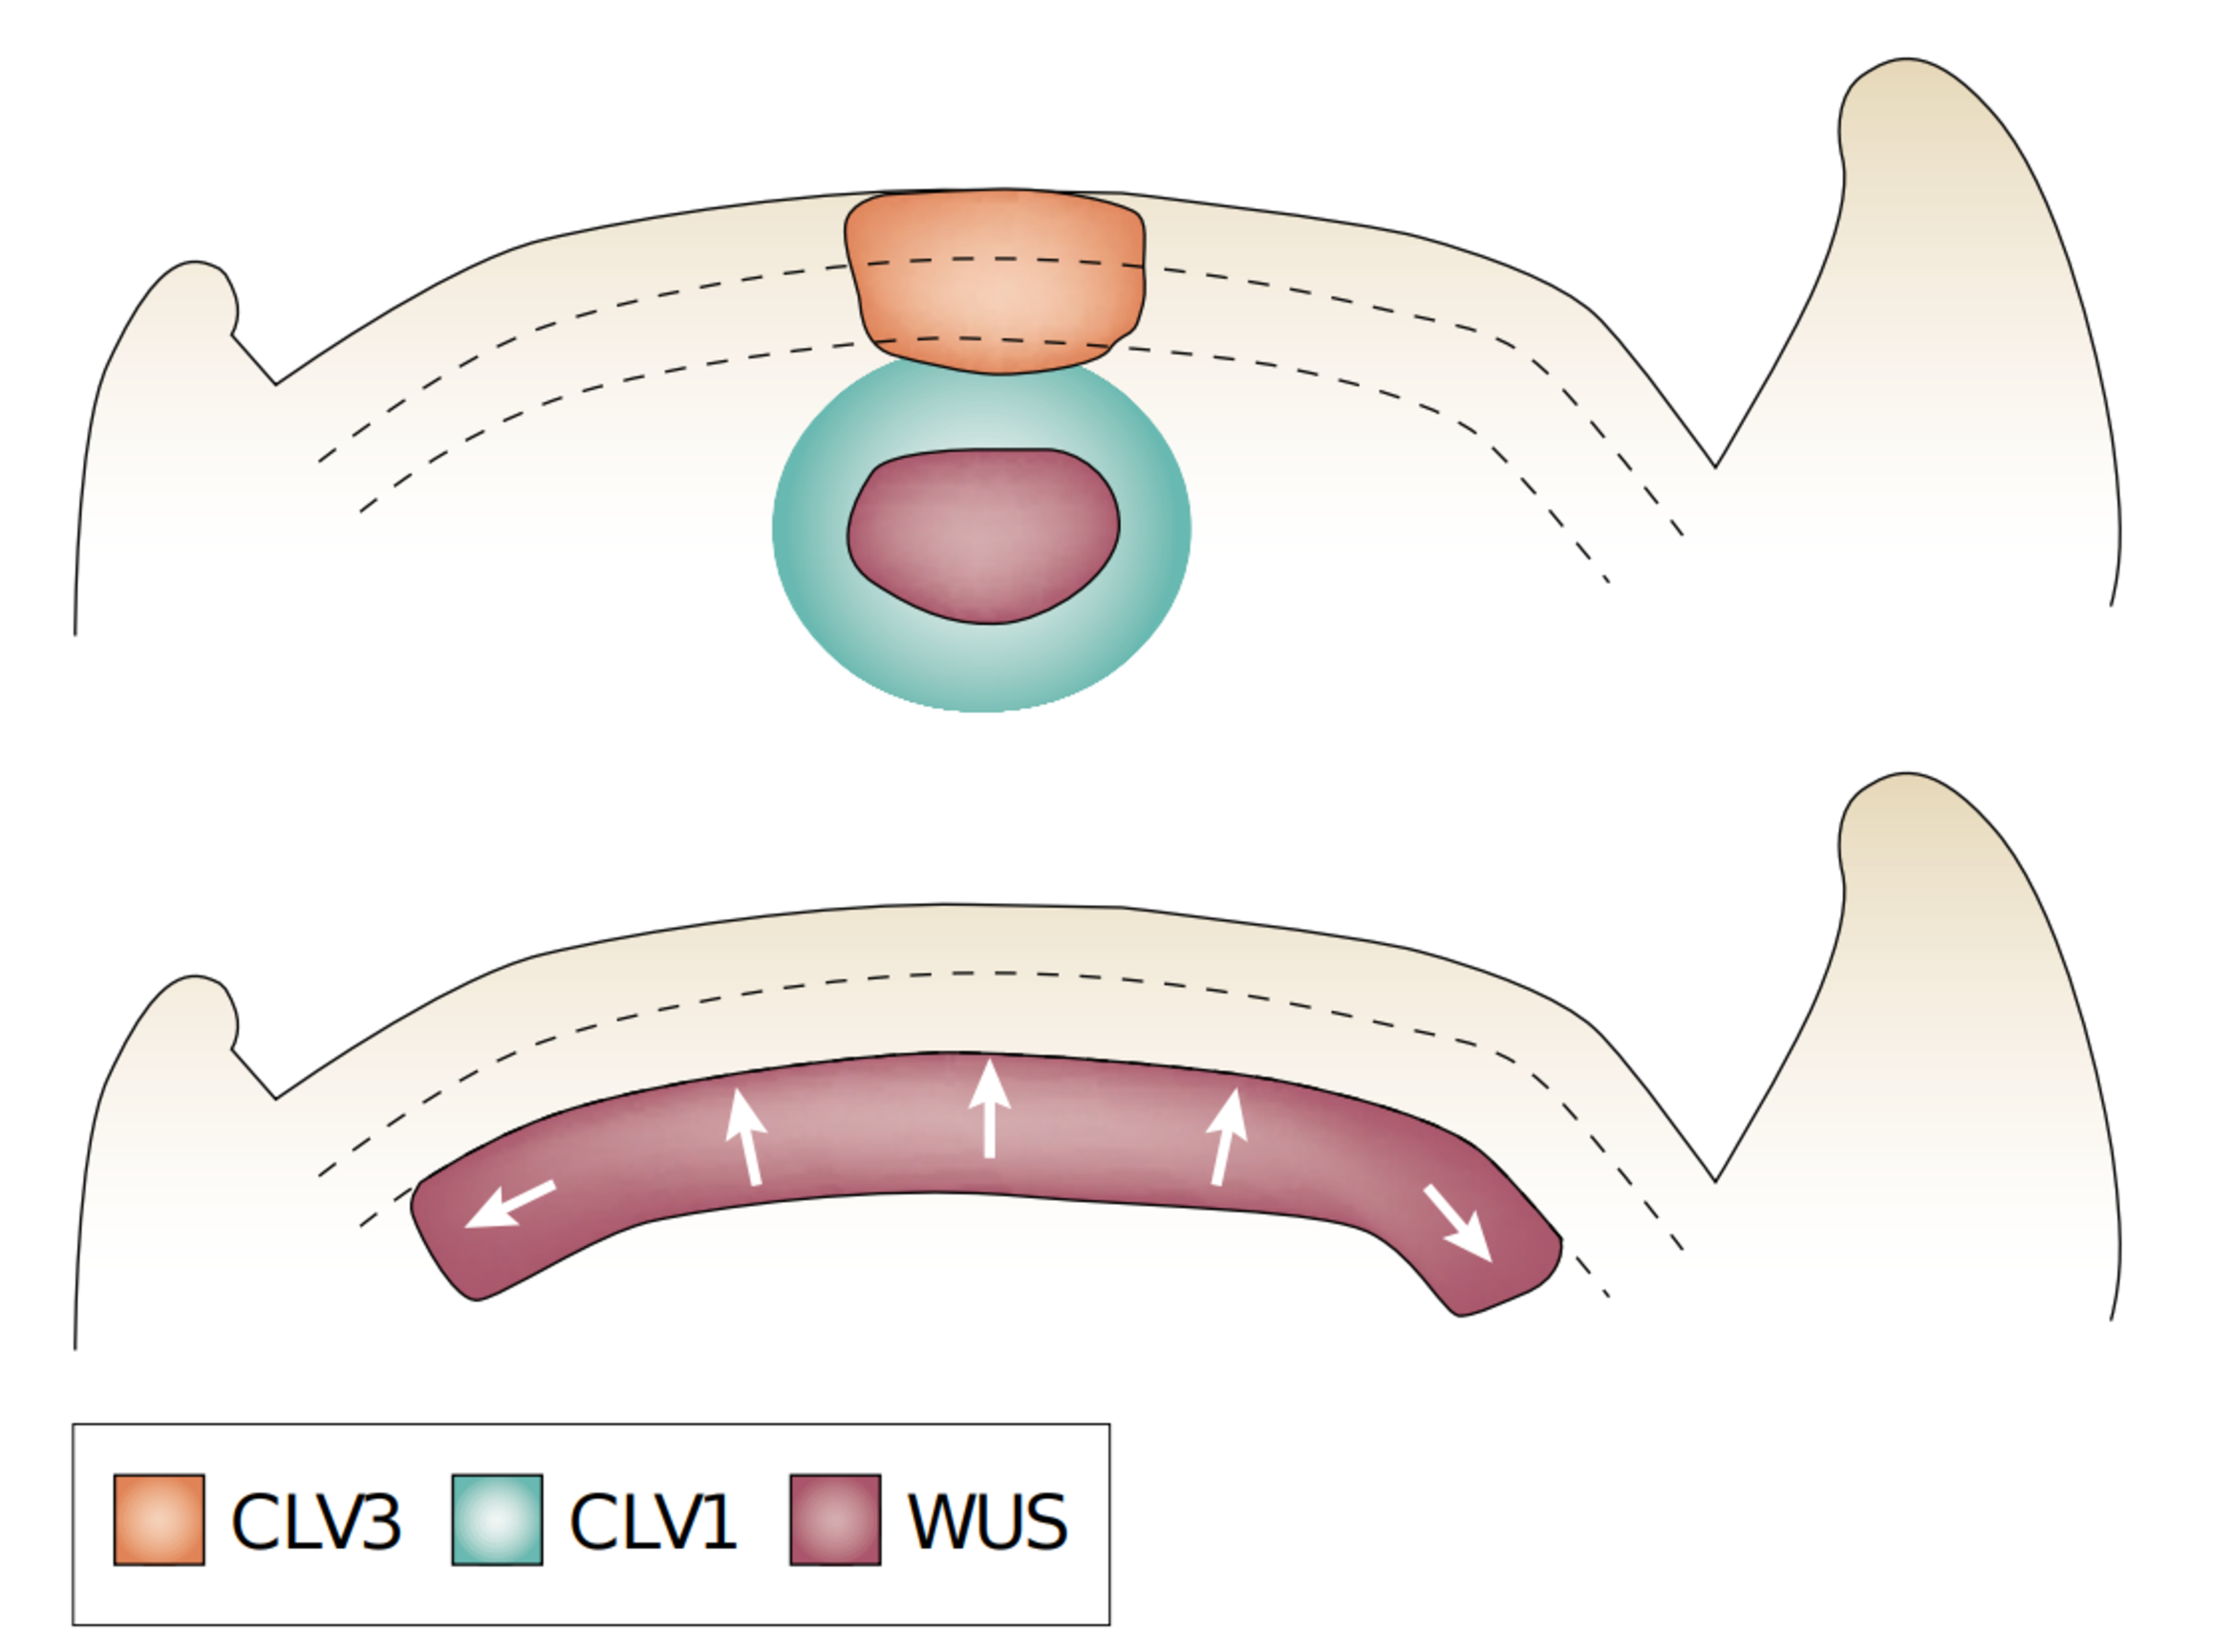
\includegraphics[width=.95\textwidth]{domains.pdf}
  \end{minipage}\hfill
  \begin{minipage}{0.45\textwidth}
    \centering
    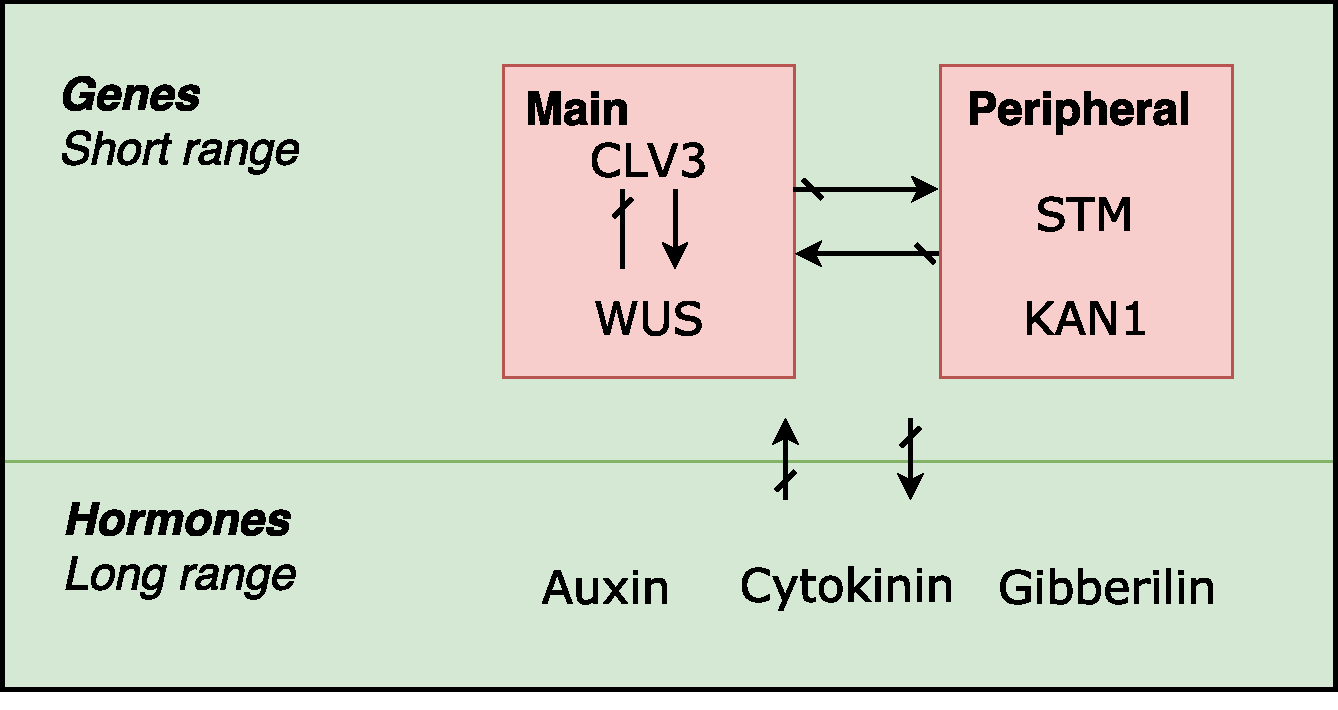
\includegraphics[width=.95\textwidth]{grn_sam.pdf} 
  \end{minipage}
  \caption[Regulation of apical stem cells]{Illustrative description of
    biochemical regulation in the shoot, where hormones are typically actively or
    passively transported to the shoot where they affect development. Genes
    instead perform short-range signalling, either through non-coding RNA or
    via their protein products. To the left is shown the regimes of a few
    key agents in the SAM. Stem cell identifier CLV3 is expressed at the
    very apex, with its corresponding receptor molecule CLV1 present in the
    OC. Together with WUS, CLV forms an dynamic feedback loop which is
    essential to maintaining a functional stem cell niche. Figure (left) partly
    adapted from Clark~\cite{clark2001cell}.}
  \label{fig:sam_grn}
\end{figure}

In contrast to CLV3, WUS agonistically  
activates the CLV pathway through diffusion of its homeobox protein. This activating
interaction makes it necessary for maintaining an appropriate stem
cell niche, and for repressing the differentation process of the cells at the
apex. This is particularly noticable in WUS loss-of-function mutants, where the
lack of the correct WUS gradient leads to defective shoots that terminate in
aberrant flat structures~\cite{laux1996wuschel}.

Together, the CLV3-WUS feedback loop forms the core of the GRN regulating stem
cell identity. Outside of the CZ, peripherally expressed genes such as KANADI
(KAN1) are instead known to promote cell
differentiation~\cite{kerstetter2001kanadi}. The core network
itself is naturally  
also affected by the activity of other genes in extension, including hormonal
intervenience on WUS by the small and diffusive hormone cytokinin, which itself
is activated by enzymes present in the meristem~\cite{hutchison2002cytokinin}.
Also other homeobox encoding genes such as \textit{Shoot Meristemless} (STM) are
essential for correct development of the shoot by activation of
CLV3~\cite{scofield2013arabidopsis}.

Aside of the system regulating the cellular identity, also other classes of
molecules  are key to the overall development.  
The plant hormone auxin in particular has been repeatedly shown to have an
essential role in the coordination of growth, both in 
signalling initiation points of new primordia and elongation of the core stem.
Because of this, auxin transport is key to asserting apical dominance in plants
through the help of active transporters such as the PIN-FORMED (PIN) family,
inhibition of this process leads to development of organless meristems.
\cite{kvrevcek2009pin}. Also other hormones such as gibberilin are well-established
signalling molecules important for SAM
development~\cite{debeaujon2000gibberellin}.

On the whole, the molecular regulation of the
development of the SAM consists of an intricate system that requires both tight
regulation and precise coordination. This allows the plant to both counter and 
utilise noise that might be present due to volatile environements, or inherent
molecular processes, so that functional and robust development can be ensured.

\section{The role of plant stem cell modelling}
An important question in developmenal biology is how organisms can have robust
development despite consisting of many independetly variable
parts~\cite{mirabet2012noise,ciliberti2007robustness,lempe2013molecular}.
At the same time, genotypically similar plants can nevertheless exhibit
significant differences in phenotype, raising the questions of how, where and
why noise impacts the development of the plant. 

Understanding the true mechanics behind meristem development could have
significant impact particularly on crop yield. Almost 80~\% of the food supply
of the modern world in some way derives from SAMs, in the form of various types
of crops~\cite{eightyperc}. Elucidating the underlying functions and mechanics of the
meristem is therefore of utmost relevance.

While plants, and AT in particular, have been studied throughly over the years,
it is not until recently where significant advances in imaging has allowed for
more fine-grained analyses both on 1) development of the plant \textit{in vivo},
and 2) the extent and regulation of noise during development. The modern
possibility of using 3D confocal microscopy to observe growth at the
single cell level has in this spirit opened the door for quantified analyses on
plant and cellular behaviour on the single cell level. Because of this, it is now
possible to expand on this using timelapses of confocal images taken under a
period to resolve not only the static image, but also the dynamic. 

Prior research has set the ground for tracking cell lineages across multiple
timepoints, although these have mainly focused on the mechanical aspects of
division and morphogenesis~\cite{willis2016cell}. In this thesis we instead use the
approaches developed in previous studies and apply them for direct biochemical
tracking of the stem cell niche on the single cell level -- an endeavour which
in itself is largely unprecedented. 

% Quantification of the SAM tissue at the single cell level\\
% Stable regulation (and regulation \textit{per se})\\
% CLV3 tracking and anisotropic growth \\
